\section{b) the Newton's method}


\subsection{Problem}

We have to find zeros of the function
\[ f(x) = -2.1 + 0.3x - xe^{-x} \]
In the interval $[-5; 10]$

using the Newton's method
\subsection{Theoretical Introduction}
\emph{The Newton's method} also called \emph{the tangent method} relies on first order part of its expansion into Taylor series for a given current approximation of root.
\[ f(x) \approx f(x_n) + f^{'}(x_n)(x-x_n) \]
Then we obtain the next point $x_{x+1}$ by finding root of linear function:
\[ f(x_n) + f^{'}(x_n)(x_{n+1}-x_n) = 0 \]
From this we get formula for $x_{n+1}$:
\[ x_{n+1} = x_n - \frac{f(x_n)}{f^{'}(x_n)} \]

This method as opposed to \emph{regula falsi} method is locally convergent, should we choose initial point too far from the root (area which is close enough to root is called set of attraction) then we can get a divergence. On the other side if the Newton's method will converge then it is quite rapid with convergence of order p = 2 - quadratic convergence.

Newton's method is also effective if the function derrivative is far from zero, so the slope of the function is steep, conversely if the derrivative is close to zero the method is not recommended.
\subsection{Results}

\begin{center}
   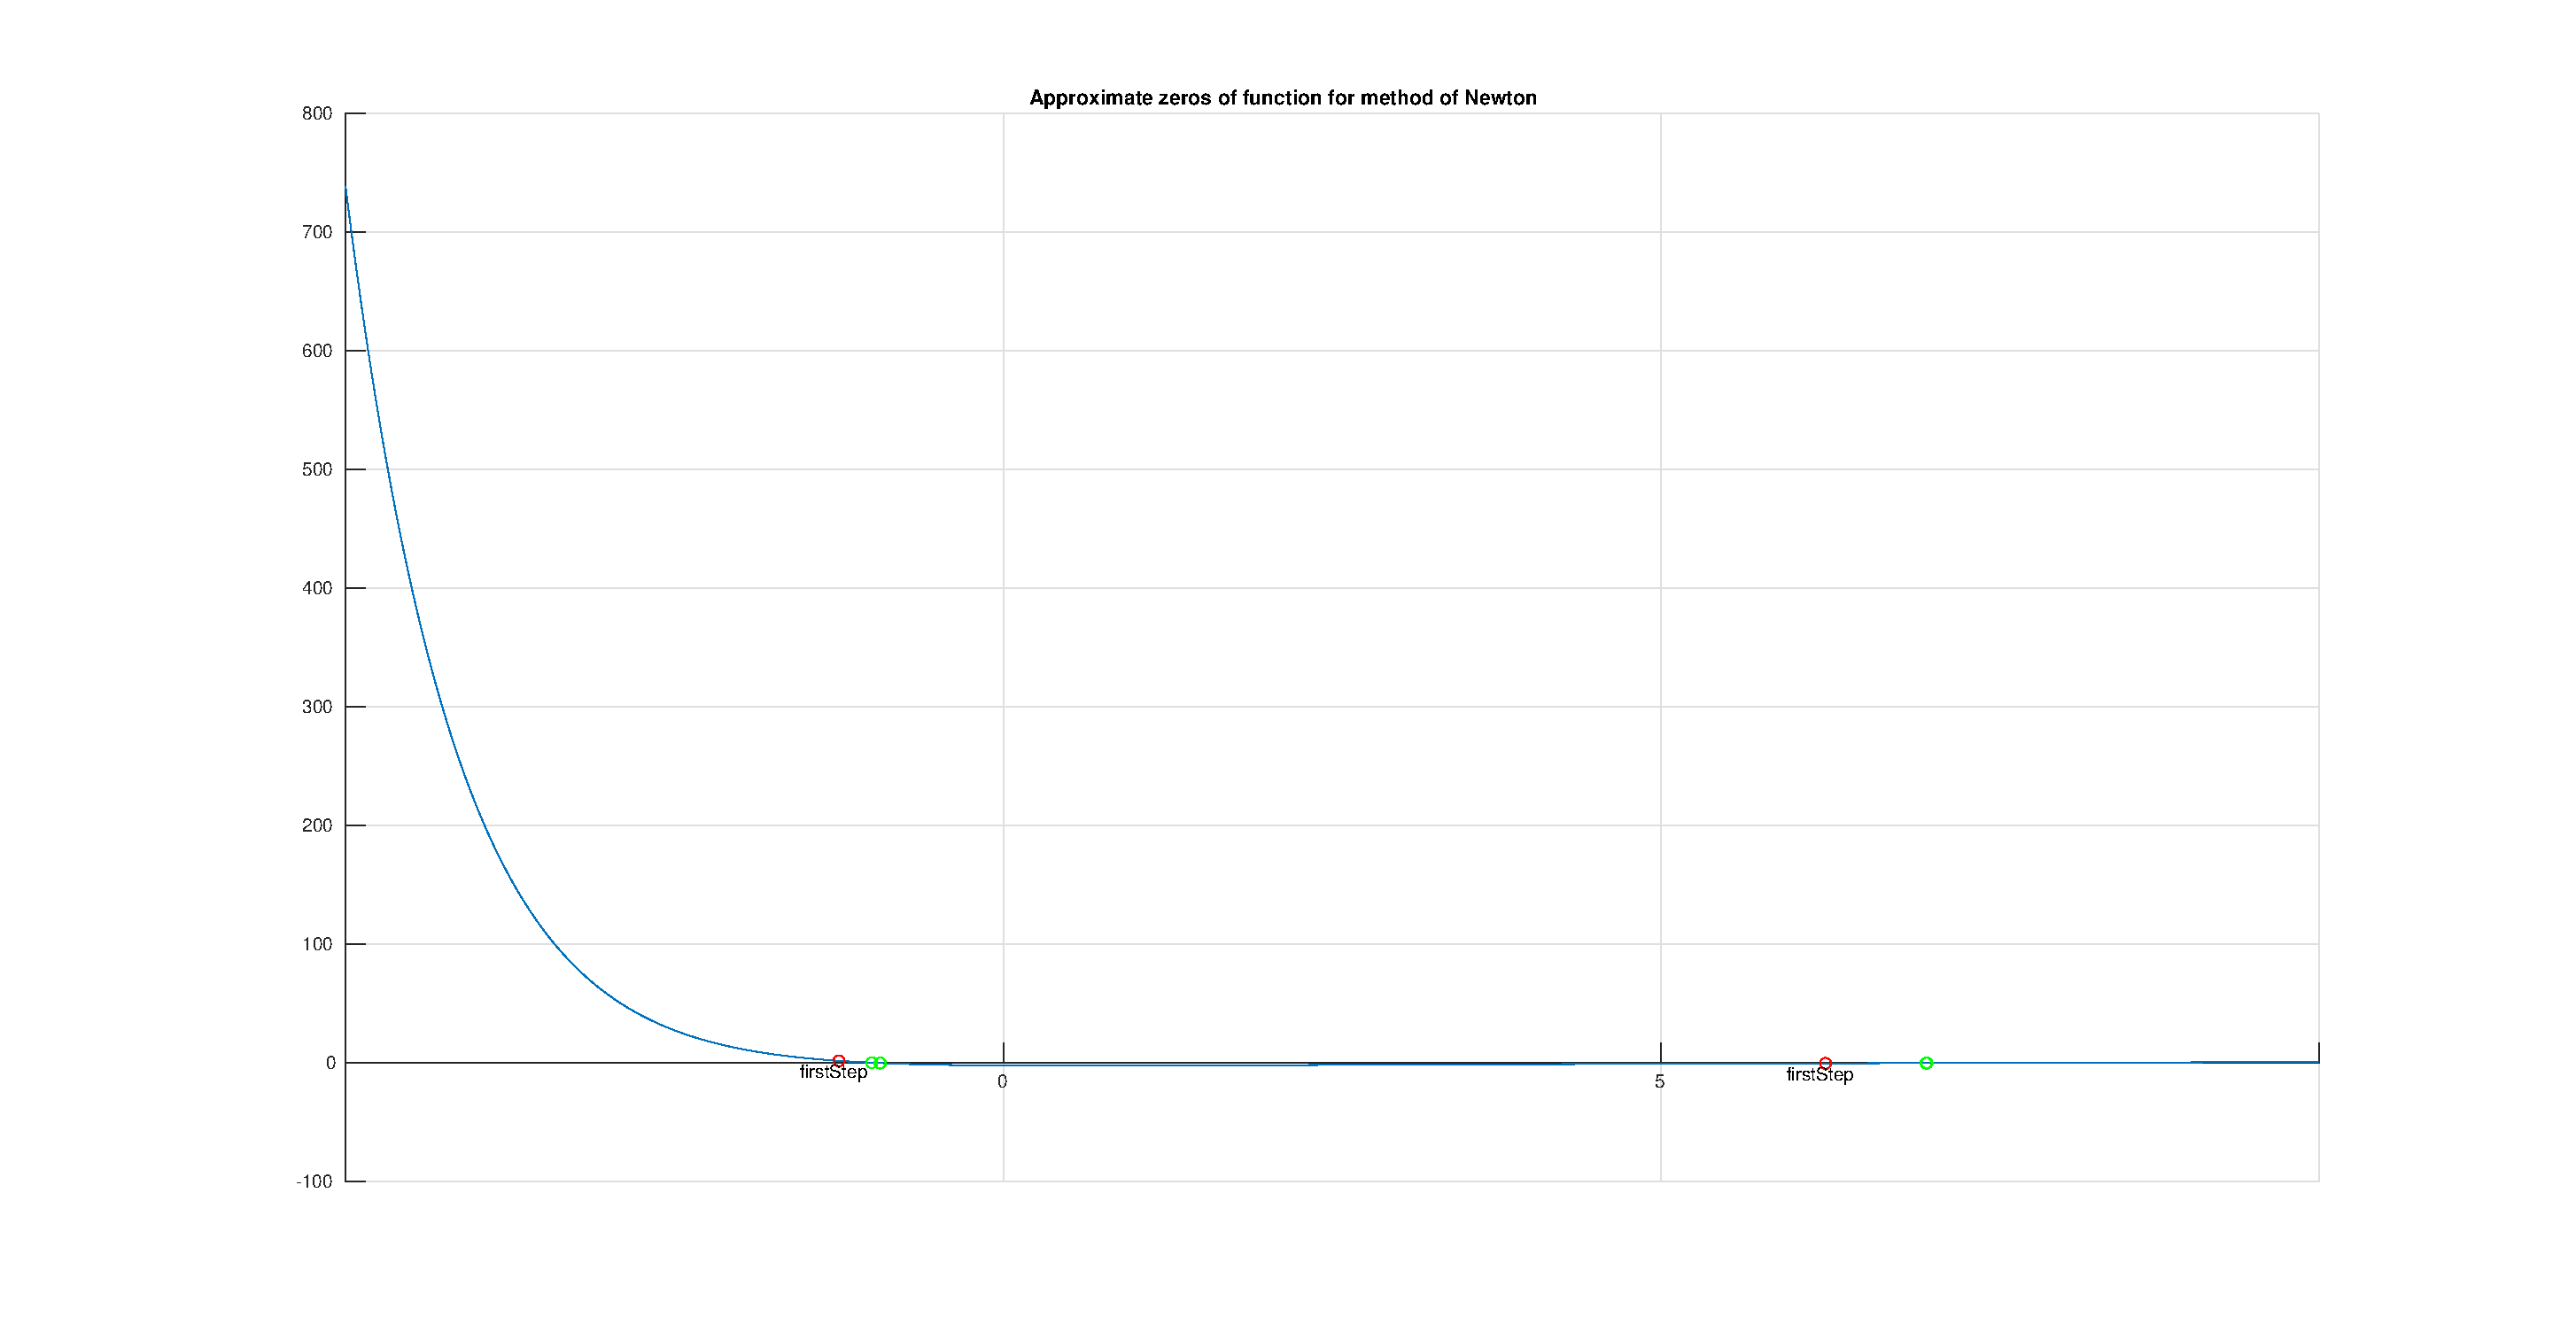
\includegraphics[scale=0.25]{task1Newtonoverall.eps}
\end{center}

\begin{center}
   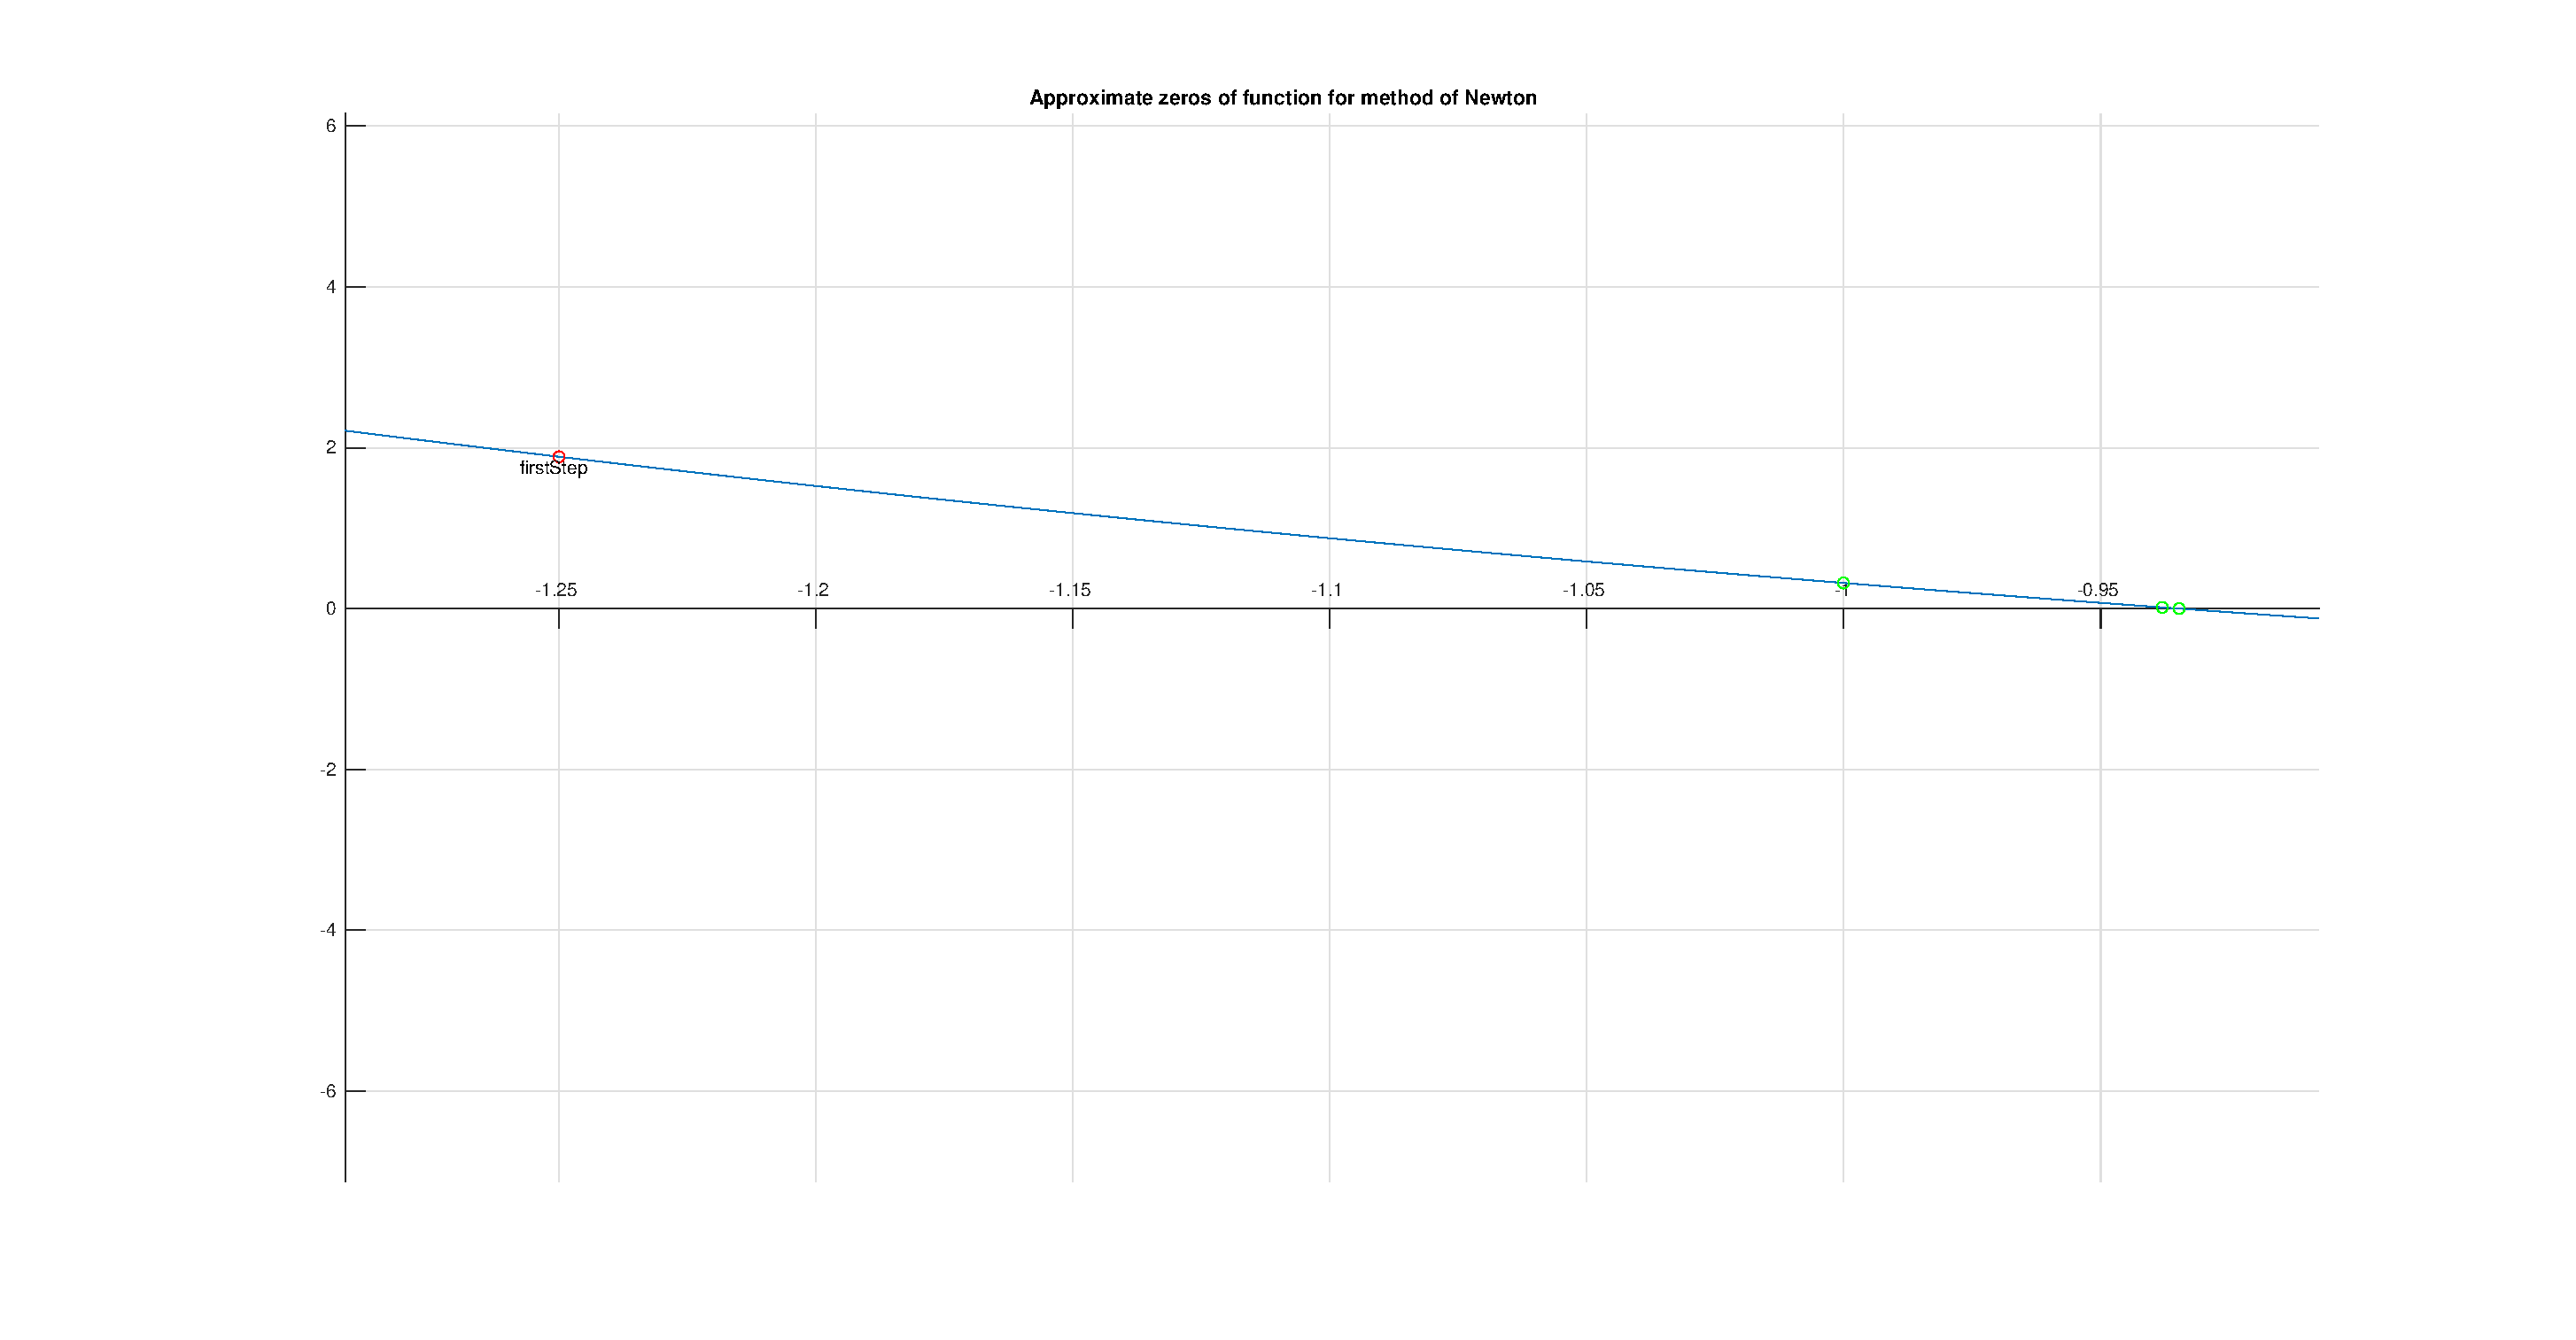
\includegraphics[scale=0.25]{task1Newtonzommedleft.eps}
\end{center}

\begin{center}
   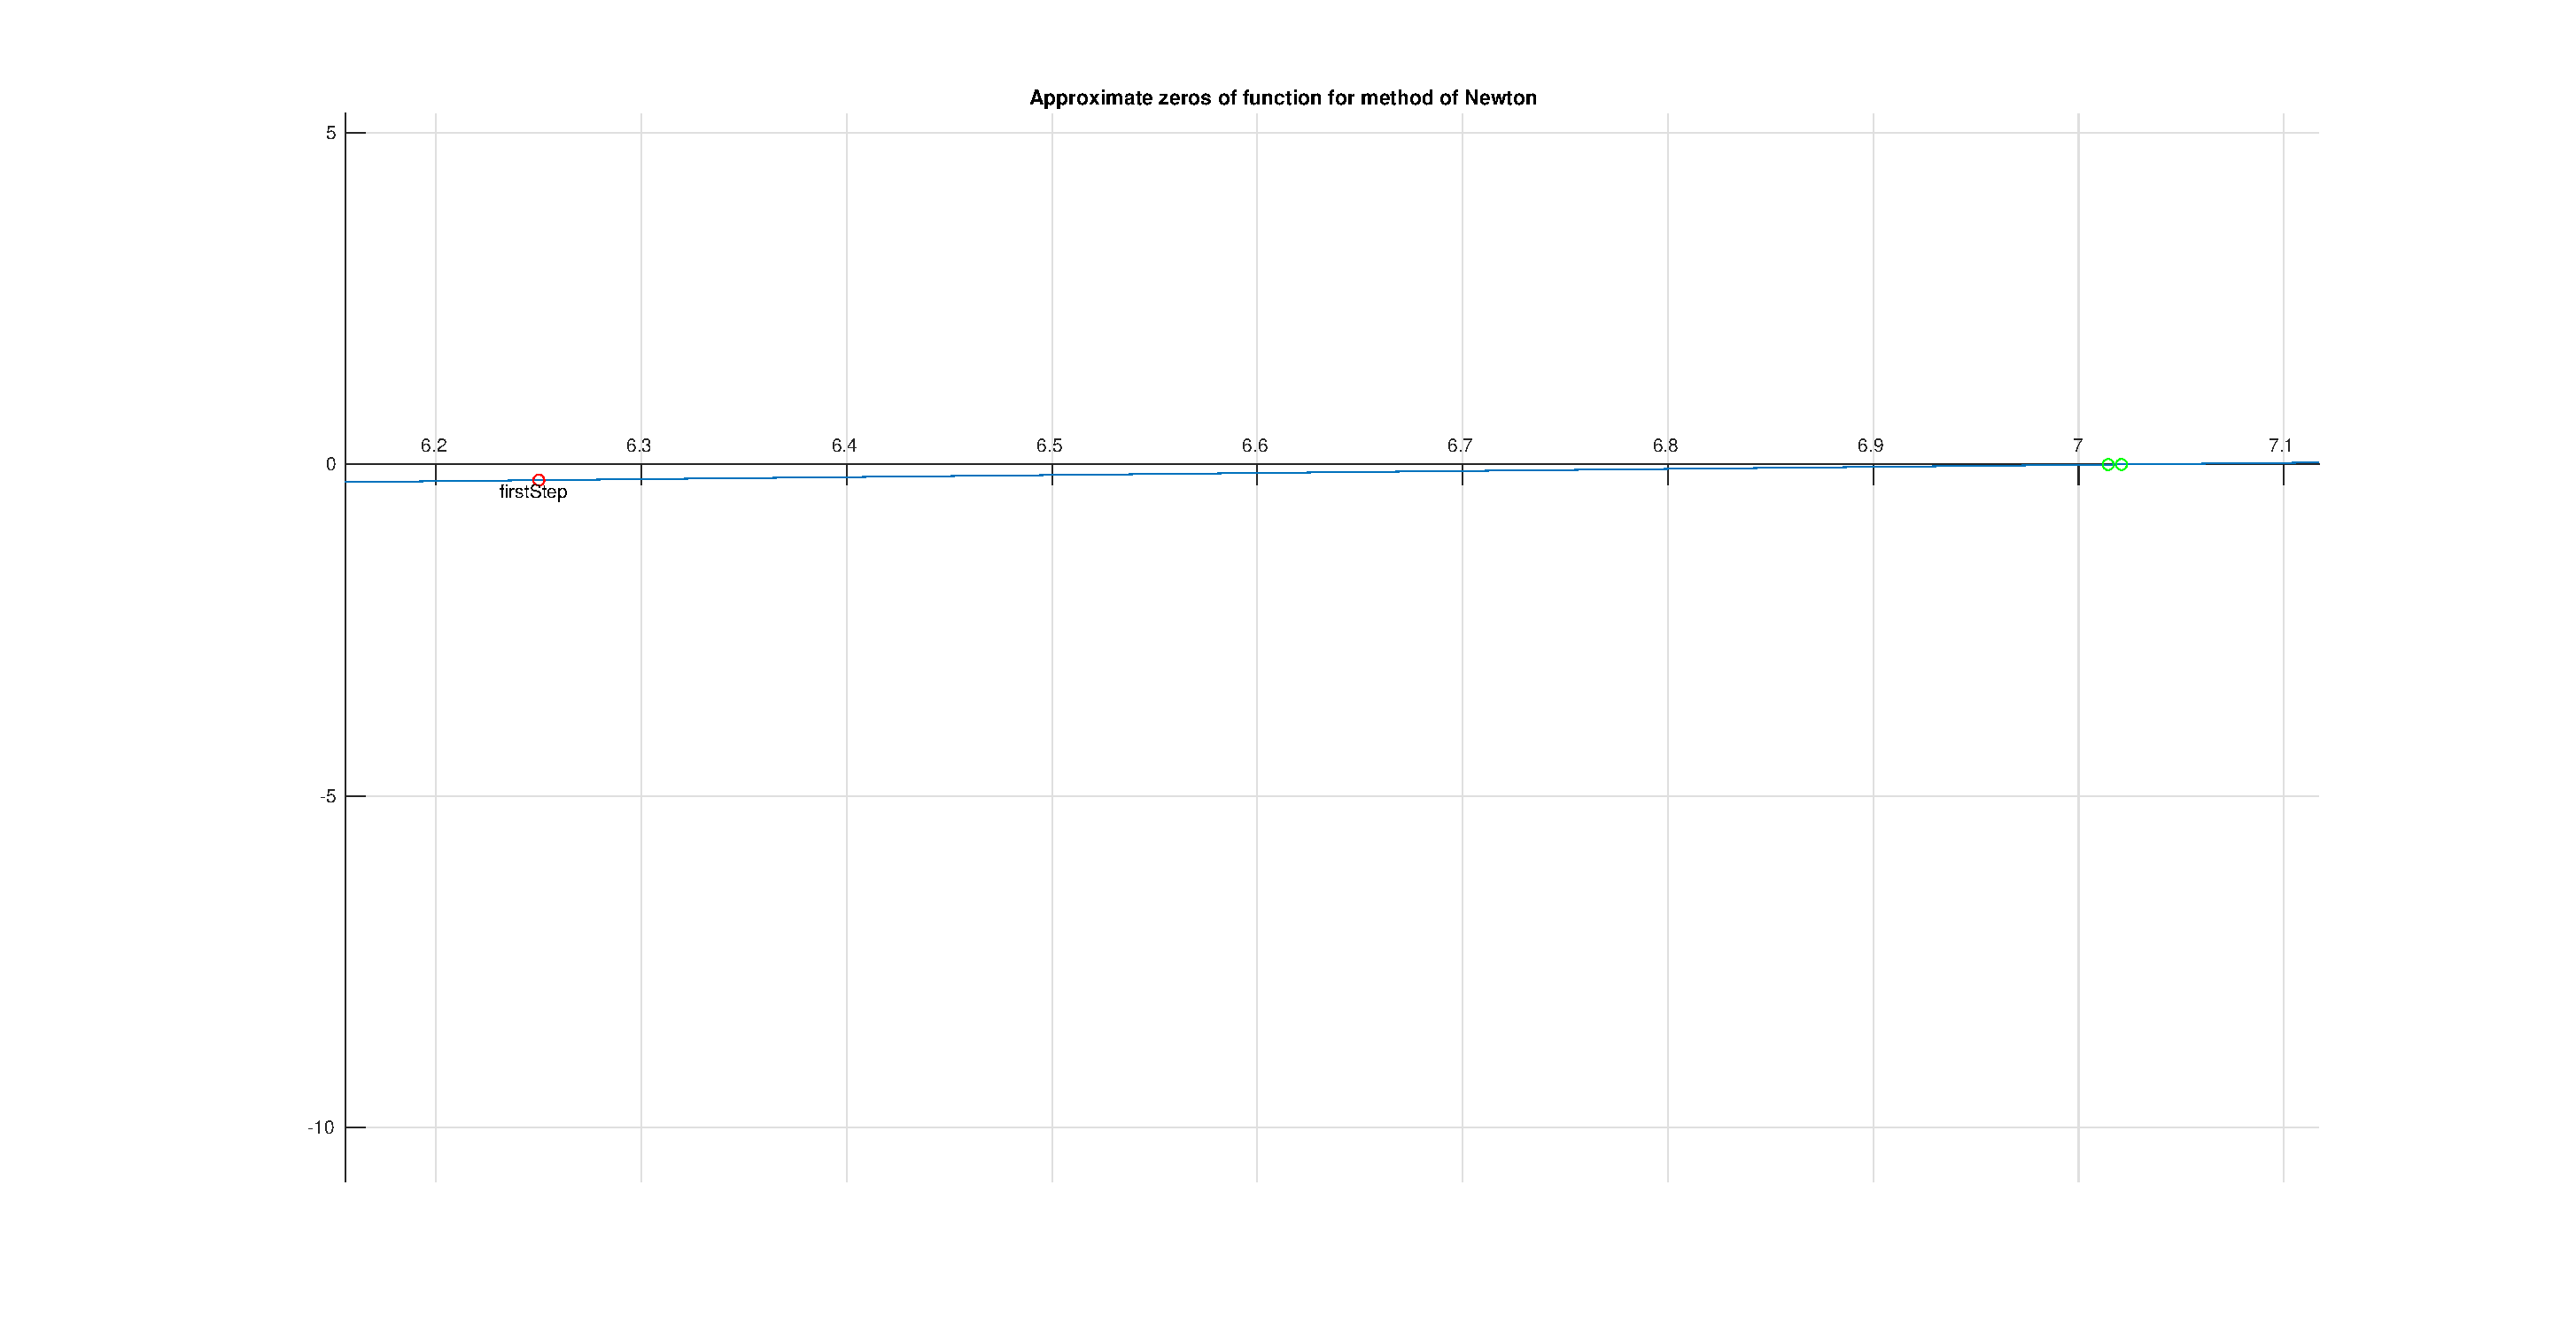
\includegraphics[scale=0.25]{task1Newtonzommedright.eps}
\end{center}

\begin{center}
  \begin{tabular}{| c  c c |}
\hline
Iteration & root         & f(root) \\
\hline
1   &      -1.25   &      1.8879  \\
\hline
2   &    -1.0001   &     0.31855  \\
\hline
3   &   -0.93804   &    0.015256  \\
\hline
4   &   -0.93476   &  4.0314e-05  \\
\hline
5   & -0.93475    & 2.8356e-10  \\
\hline
6   &   -0.93475   &           0  \\
\hline
\hline

\hline
\end{tabular}
\end{center}

\begin{center}
  \begin{tabular}{| c  c c |}
\hline
Iteration & root         & f(root) \\
\hline
1   &     6.25    &   -0.23707  \\
\hline
2    &  7.0144    & -0.0019866 \\
\hline
3     & 7.0209    & -9.517e-08  \\
\hline
4      &7.0209    &  7.468e-16  \\
\hline
\hline

\hline
\end{tabular}
\end{center}

\subsection{Discussion of results}
As we can see and as we could expect from theory Newton method reigns supreme.
It is:
\begin{enumerate}
\item Faster.
Especially for finding first root. It took 36 iterations for false position method to find first root with accuary up to $10^{-10}$ and it took only 6 iterations for the Newton method.
\item More accurate
Not only that we also got more accurate results with Newton method! With first root being so close to the real answer that the matlab calculated the value of this function at this point as exactly equal to 0. For second root the accuary is $10^{6}$ better than for the false position method.
\item Smaller gaps
Looking at graphs we got from both method we can clearly see that the gaps between the final result and each and every step are much smaller for Newton method. This again proves that it is faster and more accurate compared to false position method.
\end{enumerate}



\chapter{Find real and complex roots of the polynomial}

